\documentclass[11pt]{article}
\usepackage[margin=1in]{geometry}
\usepackage{amsmath,booktabs,graphicx,hyperref,microtype,placeins}
\title{Ditlevsen transition approximations on the Dacca likelihood benchmark}
\author{Computational-statistics benchmark note}
\date{\today}

\begin{document}
\maketitle

\section{Target and experimental design}

This experiment addresses Reviewer~1's proposed transition-density competitor
on the Dacca problem.  It distinguishes the inference grid from the evaluation
model.  A fit labeled $r=1$ uses one Ditlevsen-type transition over each monthly
observation interval; $r=20$ introduces 19 additional latent points within
each month.  Every resulting parameter vector is evaluated under the same
Euler POMP used in the DMOP manuscript, with 20 Euler substeps per month.  A
one-step Euler likelihood is not used as a measure of goodness.

The executable approximation uses the Ditlevsen--Samson (DS) second-order
conditional mean, the leading first-bracket covariance, and a disclosed
relative covariance floor of $10^{-10}$.  Its marginal Gaussian
quasi-likelihood is evaluated by an extended Kalman recursion and optimized by
projected Adam.  This deterministic QML fit is favorable in that it removes
SAEM path-imputation Monte Carlo error.  It is not labeled as the original DS
SAEM: the full Dacca state does not satisfy that paper's one-smooth-coordinate,
full-rank-rough-block structure, and its complete likelihood does not have the
closed-form curved-exponential-family M-step used in their examples.

The scaled multi-start experiment uses five starts: the published Dacca point
and four draws from the same wide physical-scale box used by the manuscript.
Each fit receives 25 projected-Adam iterations.  This is sufficient to expose
global reliability but is not represented as a reproduction of the paper's
100-search compute budget.  A separate 40-iteration run from the favorable
published point checks additional optimization.  Successful fitted vectors and
the starting point are independently evaluated with 5,000 particles and 36
particle-filter replications.  The IFAD-$0.97$ value
$-3744.17$ is copied from the authoritative manuscript table and is clearly
distinguished from newly computed values.

\section{Rank and discretization diagnostics}

The rank-deficient instantaneous diffusion is not a defect: it is the defining
hypoelliptic feature.  At the published point, successive normalized
Stratonovich-drift brackets have ranks $1,2,3,4,5,6$, so the true finite-time
Dacca transition can acquire all six active directions.  DS's model has one smooth coordinate and
$p$ rough coordinates driven by an invertible diagonal $p$-dimensional
diffusion.  It needs only the first bracket.  Dacca has one driver and needs a
longer chain.  Consequently, the first-bracket DS leading covariance has rank
at most two; this statement concerns the approximate transition covariance,
not the instantaneous diffusion rank.
In rank terms, DS assume diffusion rank $d-1$ for a $d$-state model, whereas
the active Dacca representation has $d=6$ and diffusion rank one.  An
invertible state transformation cannot remove this mismatch.
State dependence of $\sigma SI$ does not repair it: the Dacca diffusion is a
scalar field times the fixed vector $(-1,1,0,0,0,0)^\mathsf T$, so its
Milstein/diffusion-derivative terms remain collinear with that vector.  The
first drift-propagation term adds only the $J_b g$ direction.

Figure~\ref{fig:discretization} separates this structural issue from the
fine-grid mixing issue.  Ordinary one-substep backward weights become nearly
deterministic as $r$ grows.  A fixed-month linear-Gaussian endpoint-lookahead
calculation,
which supplies the multi-step marginals and bridge conditionals required by
Karppinen, Singh, and Vihola (KSV), keeps the diagnostic ESS near its maximum.
The displayed experiment uses 128 candidate parents, 500 replications, and a
parent spread equal to 0.01 times the fixed-month process standard deviation.
Repeating it at spreads 0.001 and 0.1 gives the same refinement pattern; those
results are retained in \texttt{backward\_mixing\_sensitivity.csv} and
\texttt{mixing\_sensitivity.png}.
At $r=1$ the ordinary and bridge blocks coincide; their poor diagnostic value
there is instead caused by instability of the monthly Taylor transition.

\begin{figure}[htbp]
\centering
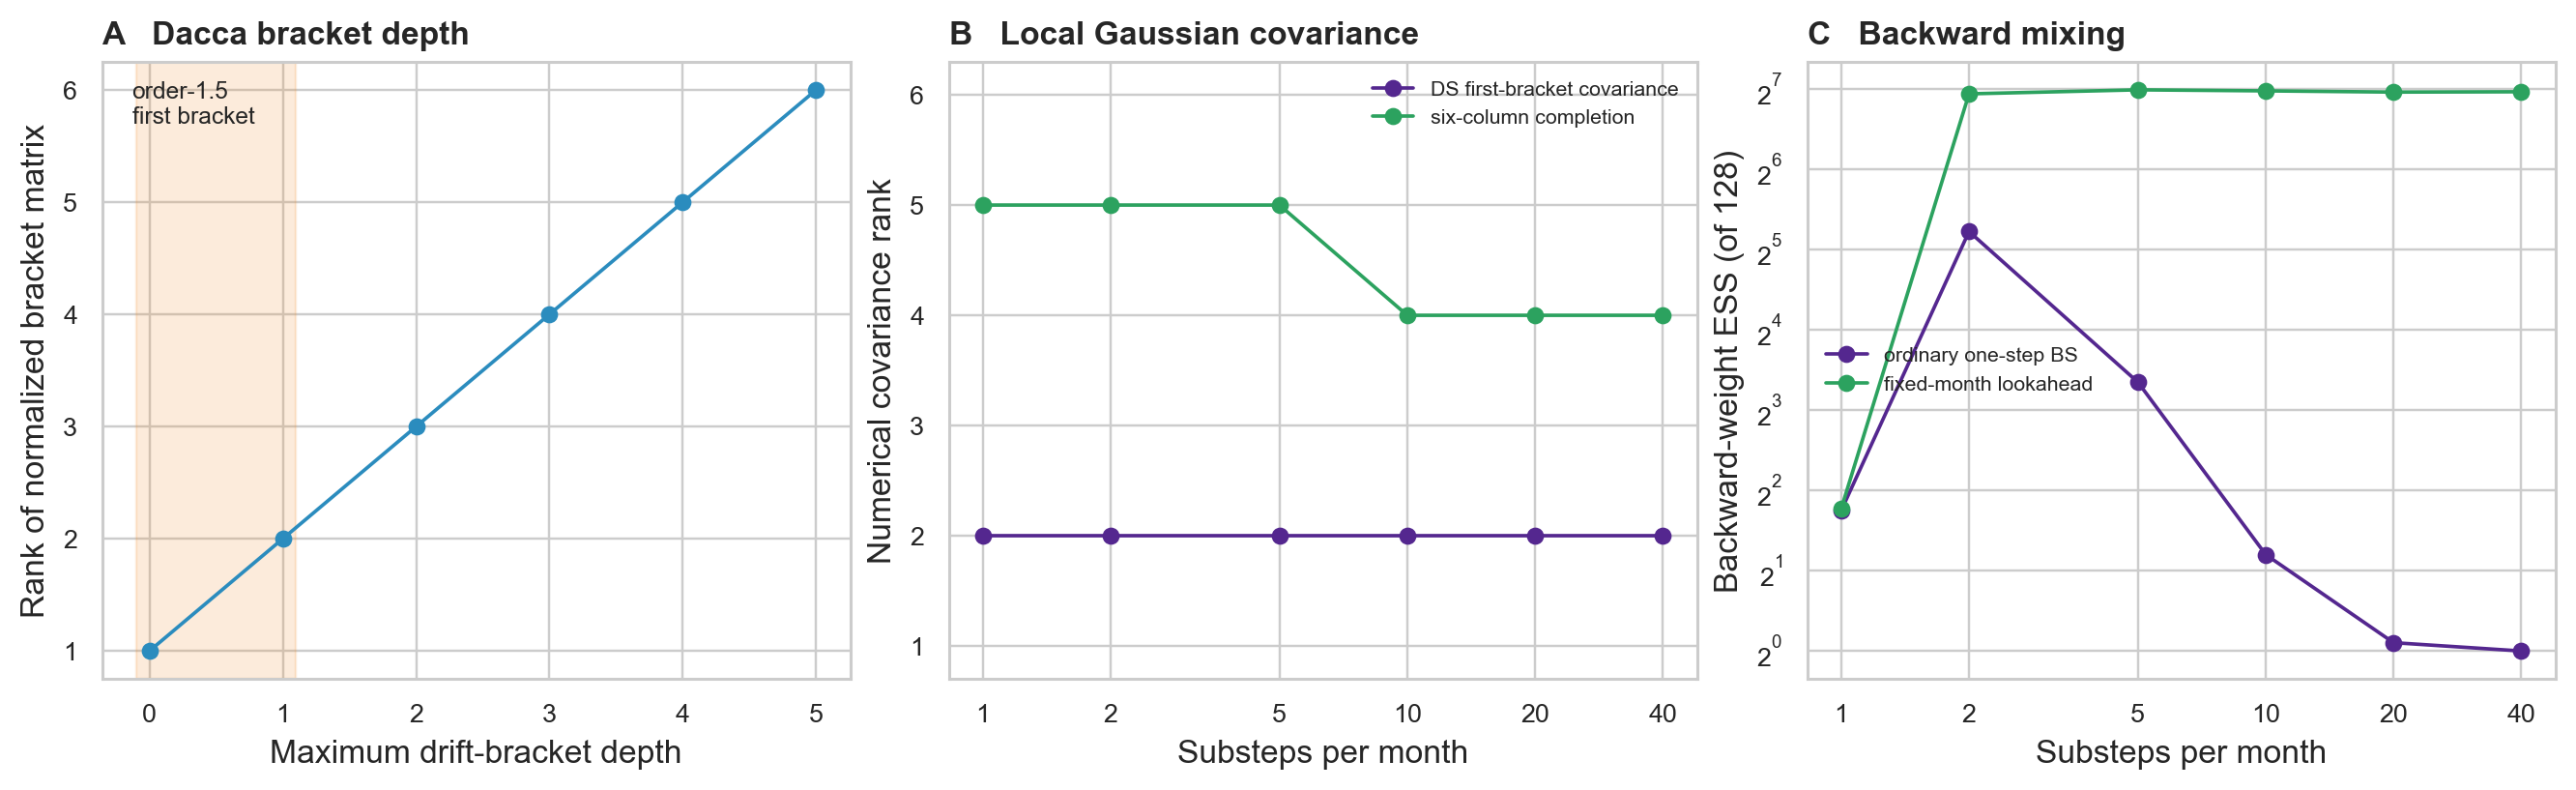
\includegraphics[width=\textwidth]{discretization_diagnostics.png}
\caption{\textbf{A:} Rank gained through successive Dacca Stratonovich-drift brackets; the
shading marks the first-bracket depth represented by the DS leading
approximation. \textbf{B:} Numerical covariance rank without a nugget.  The
six-column completion is algebraically full rank but increasingly ill
conditioned at fine steps. \textbf{C:} Effective sample size of 128 candidate
backward weights.  Ordinary unit-step backward sampling collapses under grid
refinement, whereas a fixed-month lookahead remains stable.  This is a
mechanism diagnostic, not an execution of the full CPF-BBS kernel.}
\label{fig:discretization}
\end{figure}

\FloatBarrier
\section{Parameter-estimation results}

At $r=1$ and $r=2$, the DS Taylor mean leaves the physically meaningful state
region within the first two months and the full-series Gaussian criterion
becomes non-finite.  This is a large-step stability failure, despite $r=1$
being exactly the measurement grid.  Fits become numerically available at
$r=5,10,20$.  Optimizing their own Gaussian criteria moves the favorable-start
parameters away from the high-likelihood starting point when judged by the
Euler-20 target, while the wide-box starts remain far from the target's
high-likelihood region.

This does not conflict with using the observation grid in the DS examples:
matching the measurement grid does not guarantee that the local Taylor mean is
stable for a particular model's rates.  At the published Dacca point the
three-stage immunity chain has rate $3\epsilon=57.3$ per year.  For the scalar
decay test equation, the DS second-order mean has amplification
$1-z+z^2/2$, with $z=h(3\epsilon)$.  Hence $z=4.78$ at $r=1$ and $2.39$ at
$r=2$, both outside its absolute-stability interval $0\leq z\leq2$; at $r=5$,
$z=0.96$.  This predicts the observed $r=1,2$ failure boundary.

\begin{figure}[htbp]
\centering
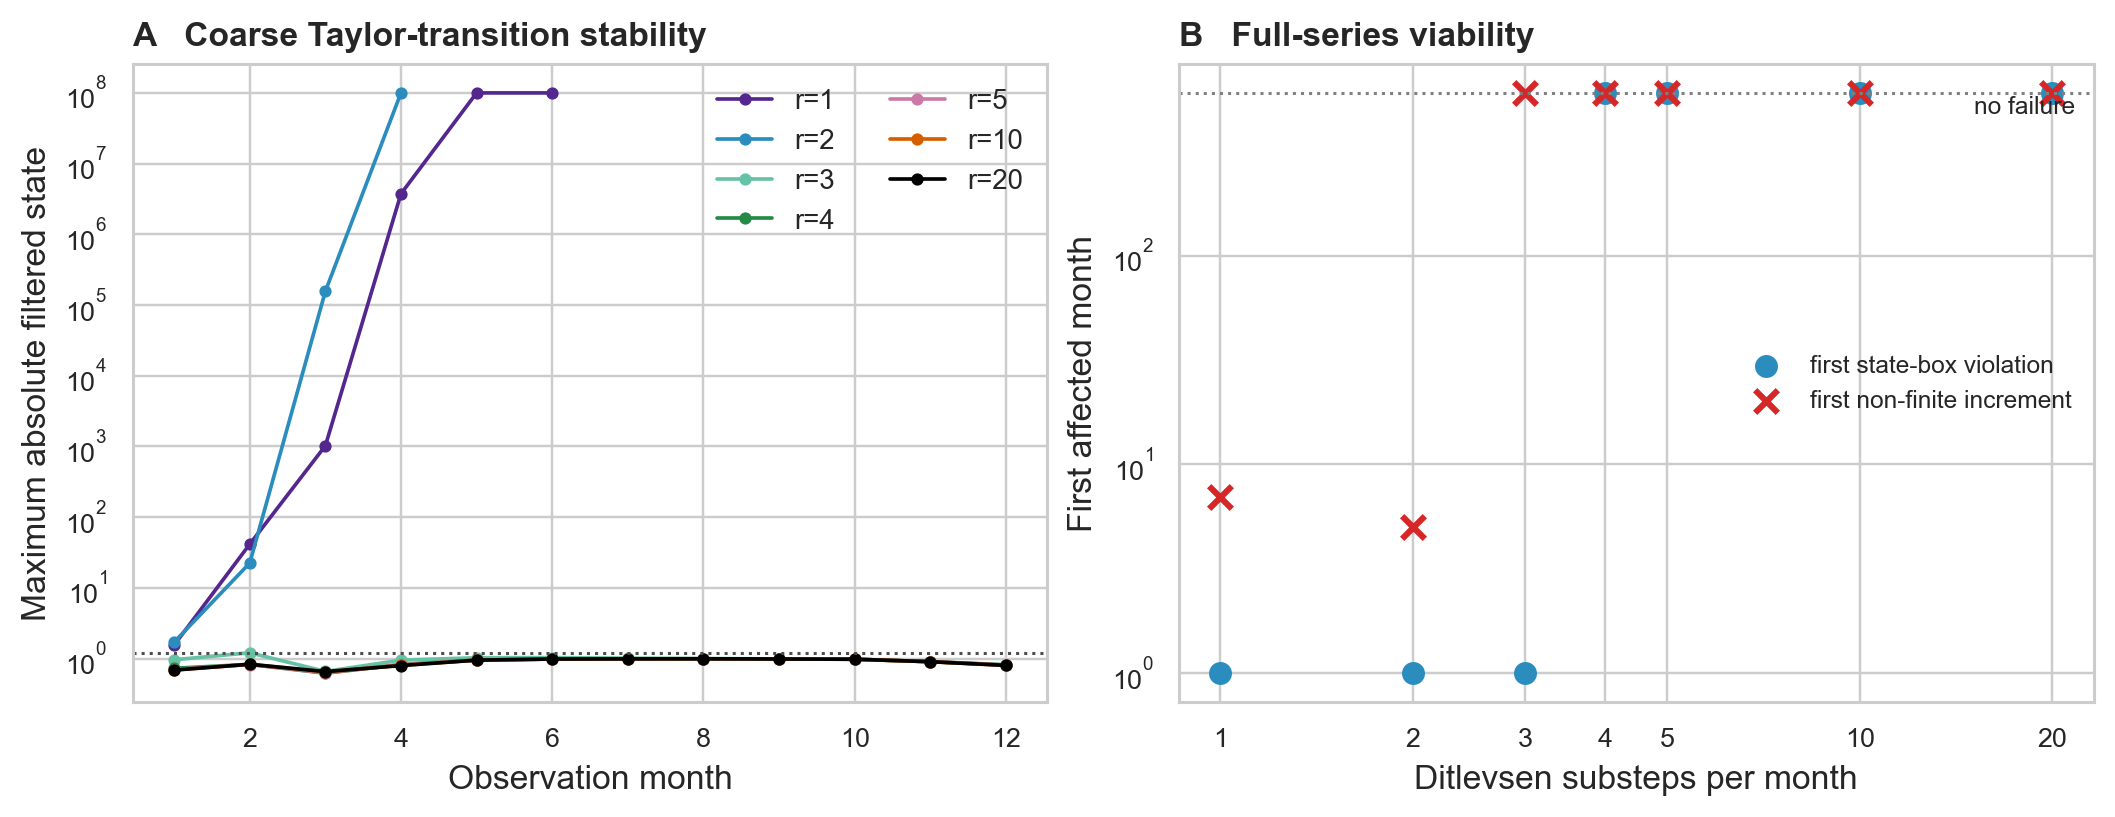
\includegraphics[width=0.94\textwidth]{taylor_stability.png}
\caption{Large-step behavior of the DS second-order Taylor mean within the
Gaussian filter.  The horizontal dotted line in panel A marks the state-box
threshold used by the fitting criterion.  Points at ``no failure'' in panel B
mean the complete 600-month recursion remained finite.}
\label{fig:stability}
\end{figure}

\begin{table}[htbp]
\centering
\begin{tabular}{rrrrr}
\toprule
DS substeps & Attempts & Successful & Best Euler-20 & Median Euler-20 \\
\midrule
1 & 5 & 0 & -- & -- \\
2 & 5 & 0 & -- & -- \\
5 & 5 & 5 & -3754.33 & -5937.07 \\
10 & 5 & 5 & -3753.86 & -5913.90 \\
20 & 5 & 5 & -3754.06 & -5913.45 \\
\midrule
\multicolumn{3}{l}{Published parameter point (reevaluated)} & -3747.95 & -- \\
\multicolumn{3}{l}{IFAD-0.97 (paper)} & -3744.17 & -3745.77 \\
\bottomrule
\end{tabular}

\caption{Fitting success and independent Euler-20 likelihood evaluation.  A
dash denotes that the DS fitting criterion was non-finite, not a missing
particle-filter evaluation.}
\label{tab:results}
\end{table}

\FloatBarrier
For the favorable published-point start, the 25-iteration Euler-20 scores at
$r=5,10,20$ are $-3754.33$, $-3753.86$, and $-3754.06$.  Continuing the same
Gaussian-surrogate optimization to 40 iterations changes them to $-3761.53$,
$-3760.41$, and $-3759.28$, respectively.  Thus improved optimization of the
DS criterion moves systematically in the wrong direction for the target
likelihood; the result is not explained by stopping the surrogate optimizer a
few iterations too early.

The successful 25-iteration scores are not monotonically worse from
$r=5$ to $r=20$; their favorable-start values are essentially flat relative to
their gap from IFAD.  This is \emph{not evidence of the opposite claim}, namely
that DS improves with grid refinement.  It means the deterministic QML wrapper
does not test the proposed SAEM path-degeneracy effect: it has no sampled latent
path whose genealogy can degenerate.  The anticipated refinement degradation
is instead seen directly in the ordinary backward-weight ESS: approximately
37.4, 10.2, 2.3, 1.07, and 1.00 out of 128 at $r=2,5,10,20,40$.
Establishing whether that mixing loss produces monotonically worse final DS-SAEM
parameter estimates requires running the full path-sampling algorithm.  The
present parameter experiment neither establishes nor refutes that monotone
ordering.

\begin{figure}[htbp]
\centering
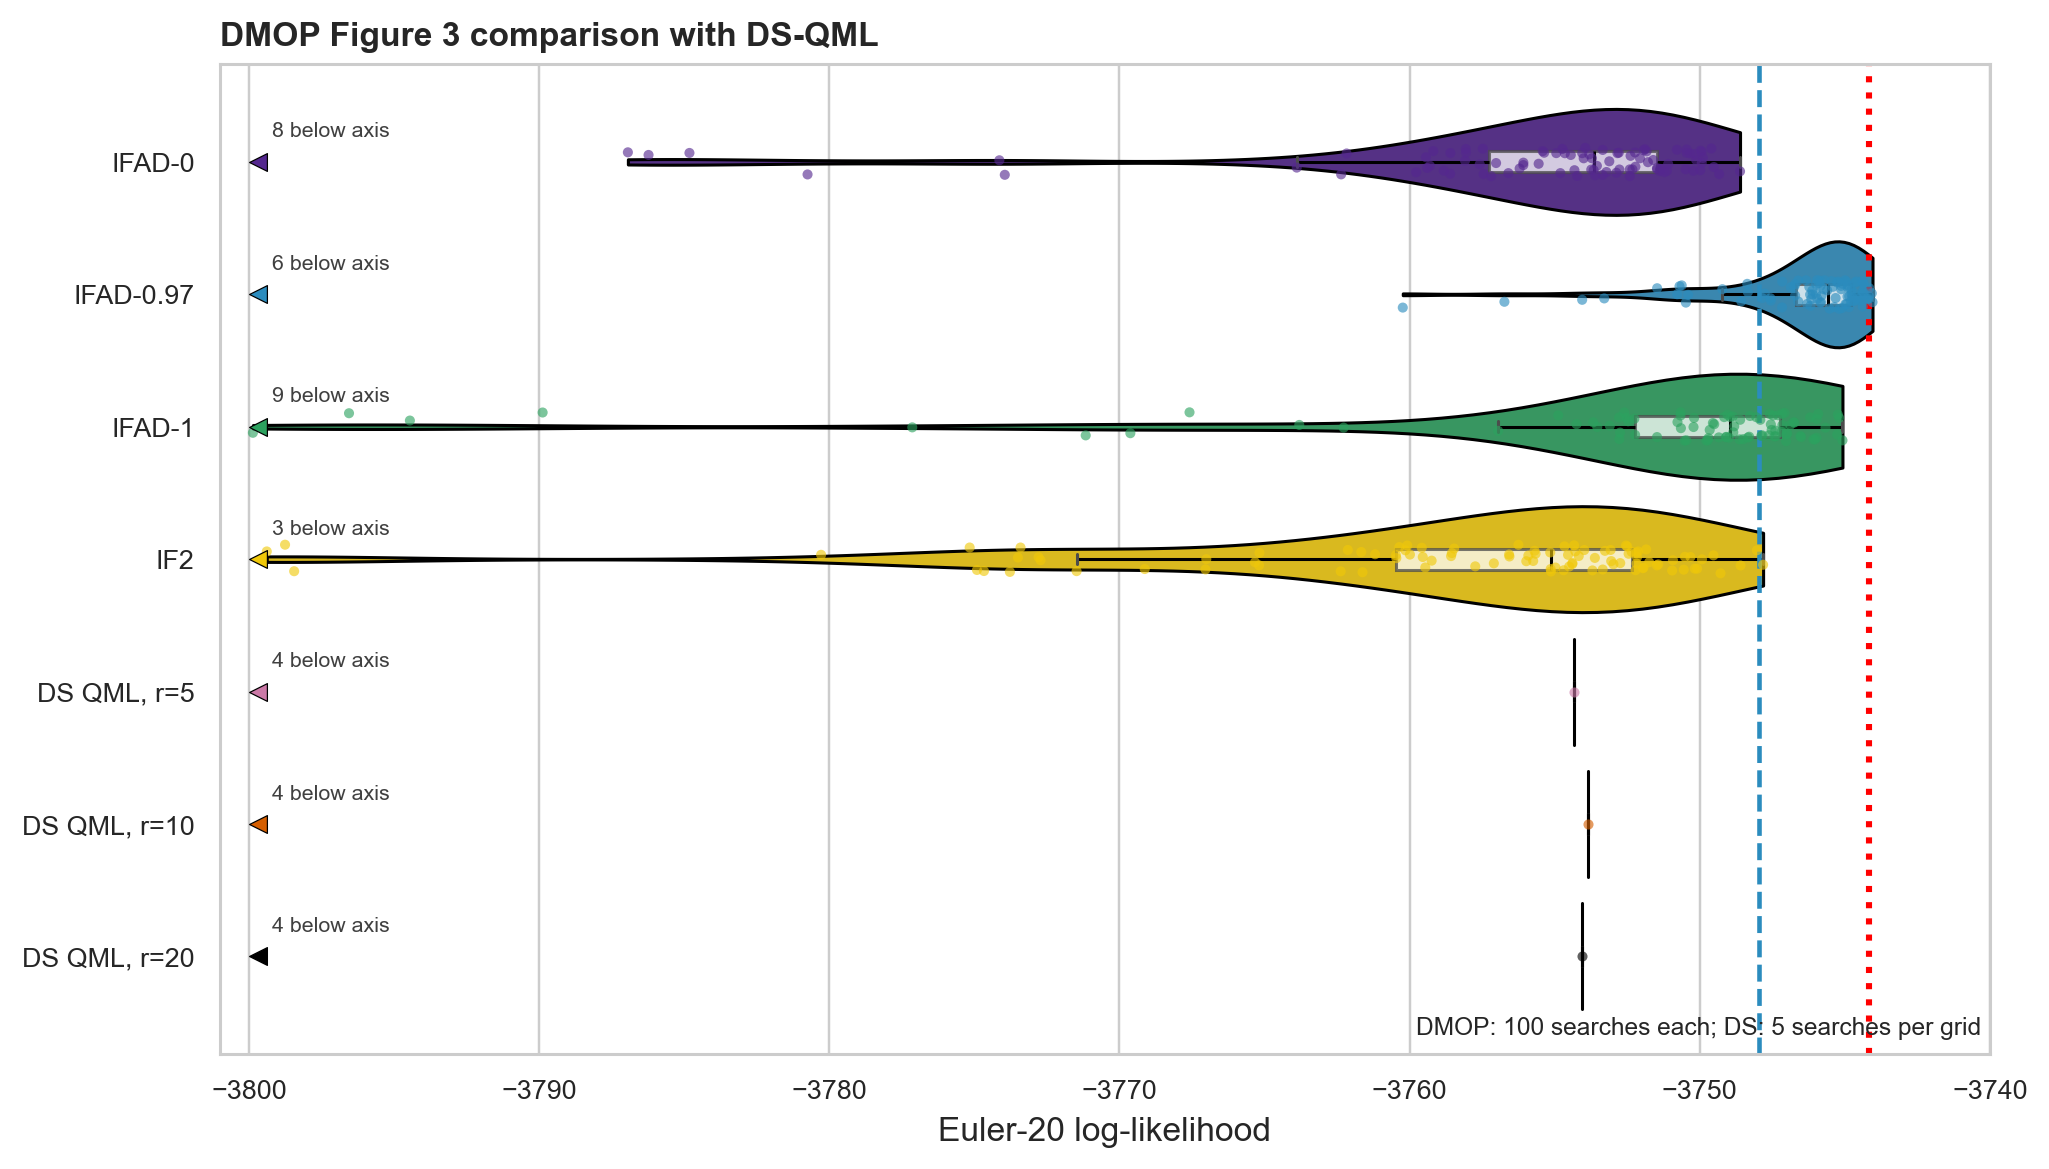
\includegraphics[width=\textwidth]{method_likelihood_comparison.png}
\caption{Analogue of DMOP Figure~3 with DS-QML added.  The four original
methods use the exact 100-search comparable-effort result objects underlying
the manuscript figure; DS has five searches per inference grid.  Values below
$-3800$ are counted at the left boundary.  The dotted red line is the paper's
best comparable-effort IFAD-$0.97$ result, and the dashed blue line is the
independently reevaluated published Dacca point.  Every DS score is evaluated
under the common Euler-20 target.}
\label{fig:likelihood}
\end{figure}

The six-column local controllability completion was also fit from the published
point at $r=5,10,20$.  This is an explicitly new higher-bracket approximation,
not DS's order-1.5 method.  Figure~\ref{fig:completion} checks whether merely
filling the omitted directions changes the Euler-20 conclusion.  Its scores
are $-3754.00$, $-3754.12$, and $-3754.06$: relative to the corresponding
first-bracket fits, changes are $+0.32$, $-0.27$, and $-0.00$ log-likelihood
units.  Thus algebraically completing the local covariance does not close the
gap to IFAD.

\begin{figure}[htbp]
\centering
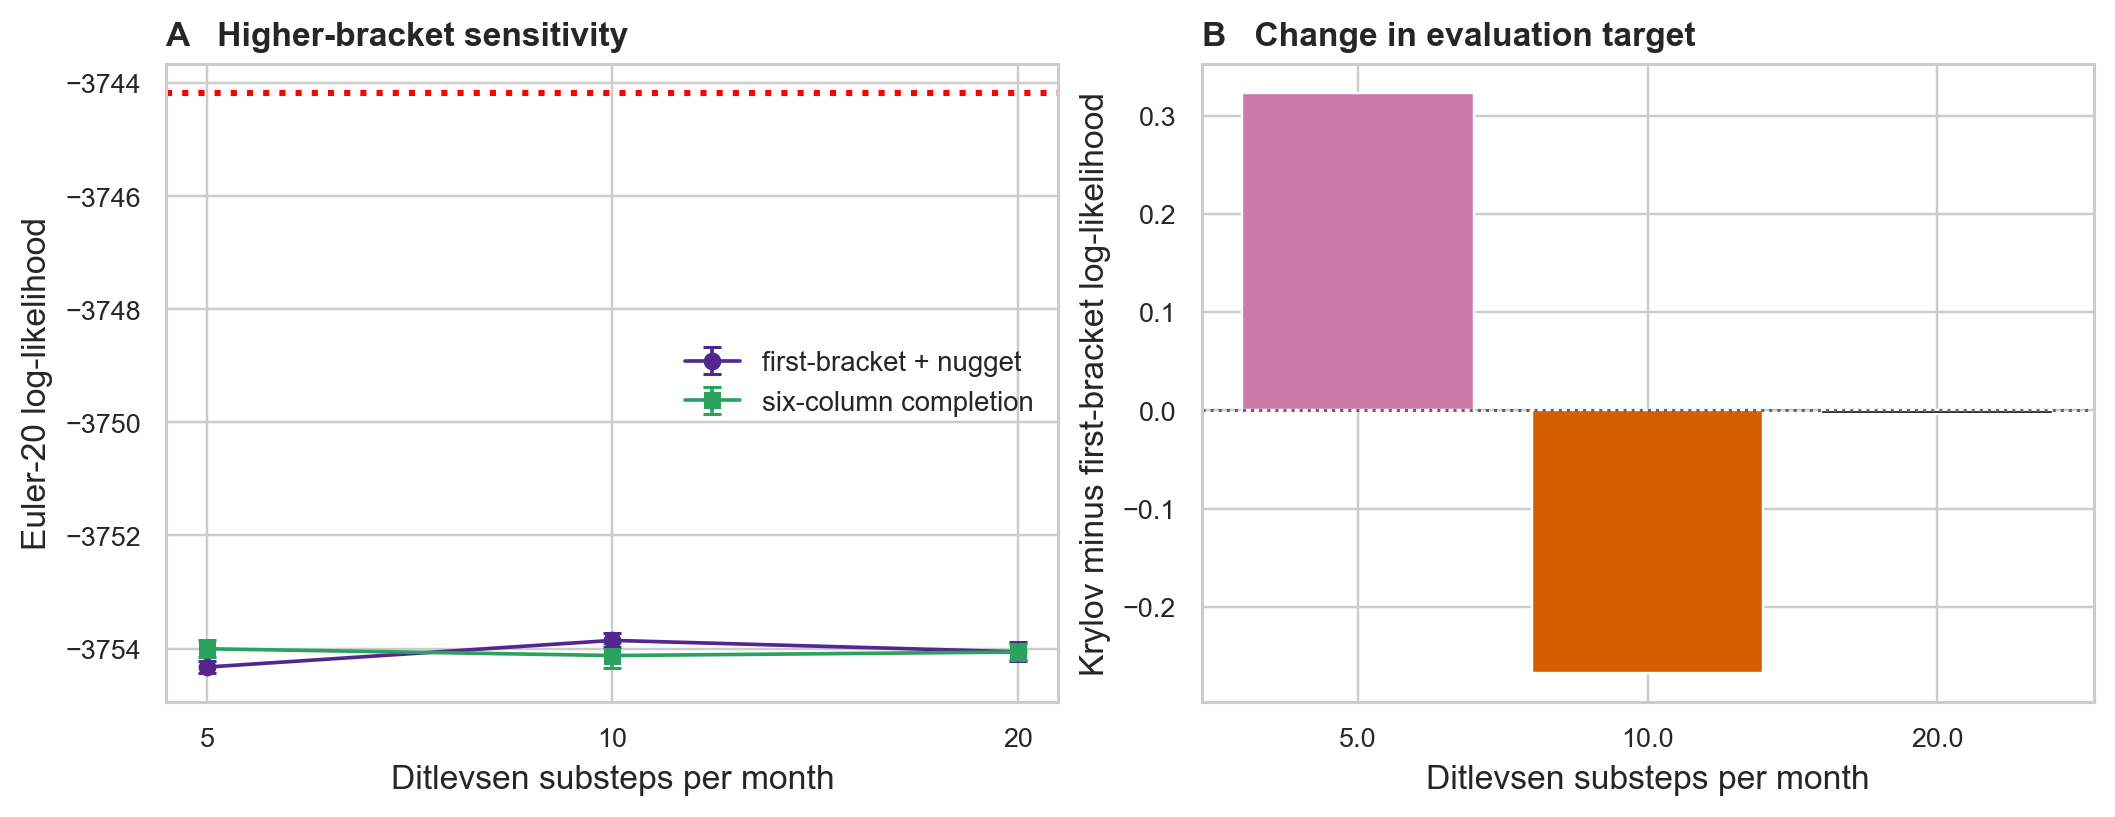
\includegraphics[width=0.94\textwidth]{completion_comparison.png}
\caption{Independent Euler-20 evaluations after fitting the first-bracket
covariance and the six-column local controllability completion from the same
published parameter point for 25 optimizer iterations.  Error bars are
particle-filter Monte Carlo standard errors.}
\label{fig:completion}
\end{figure}

\begin{figure}[htbp]
\centering
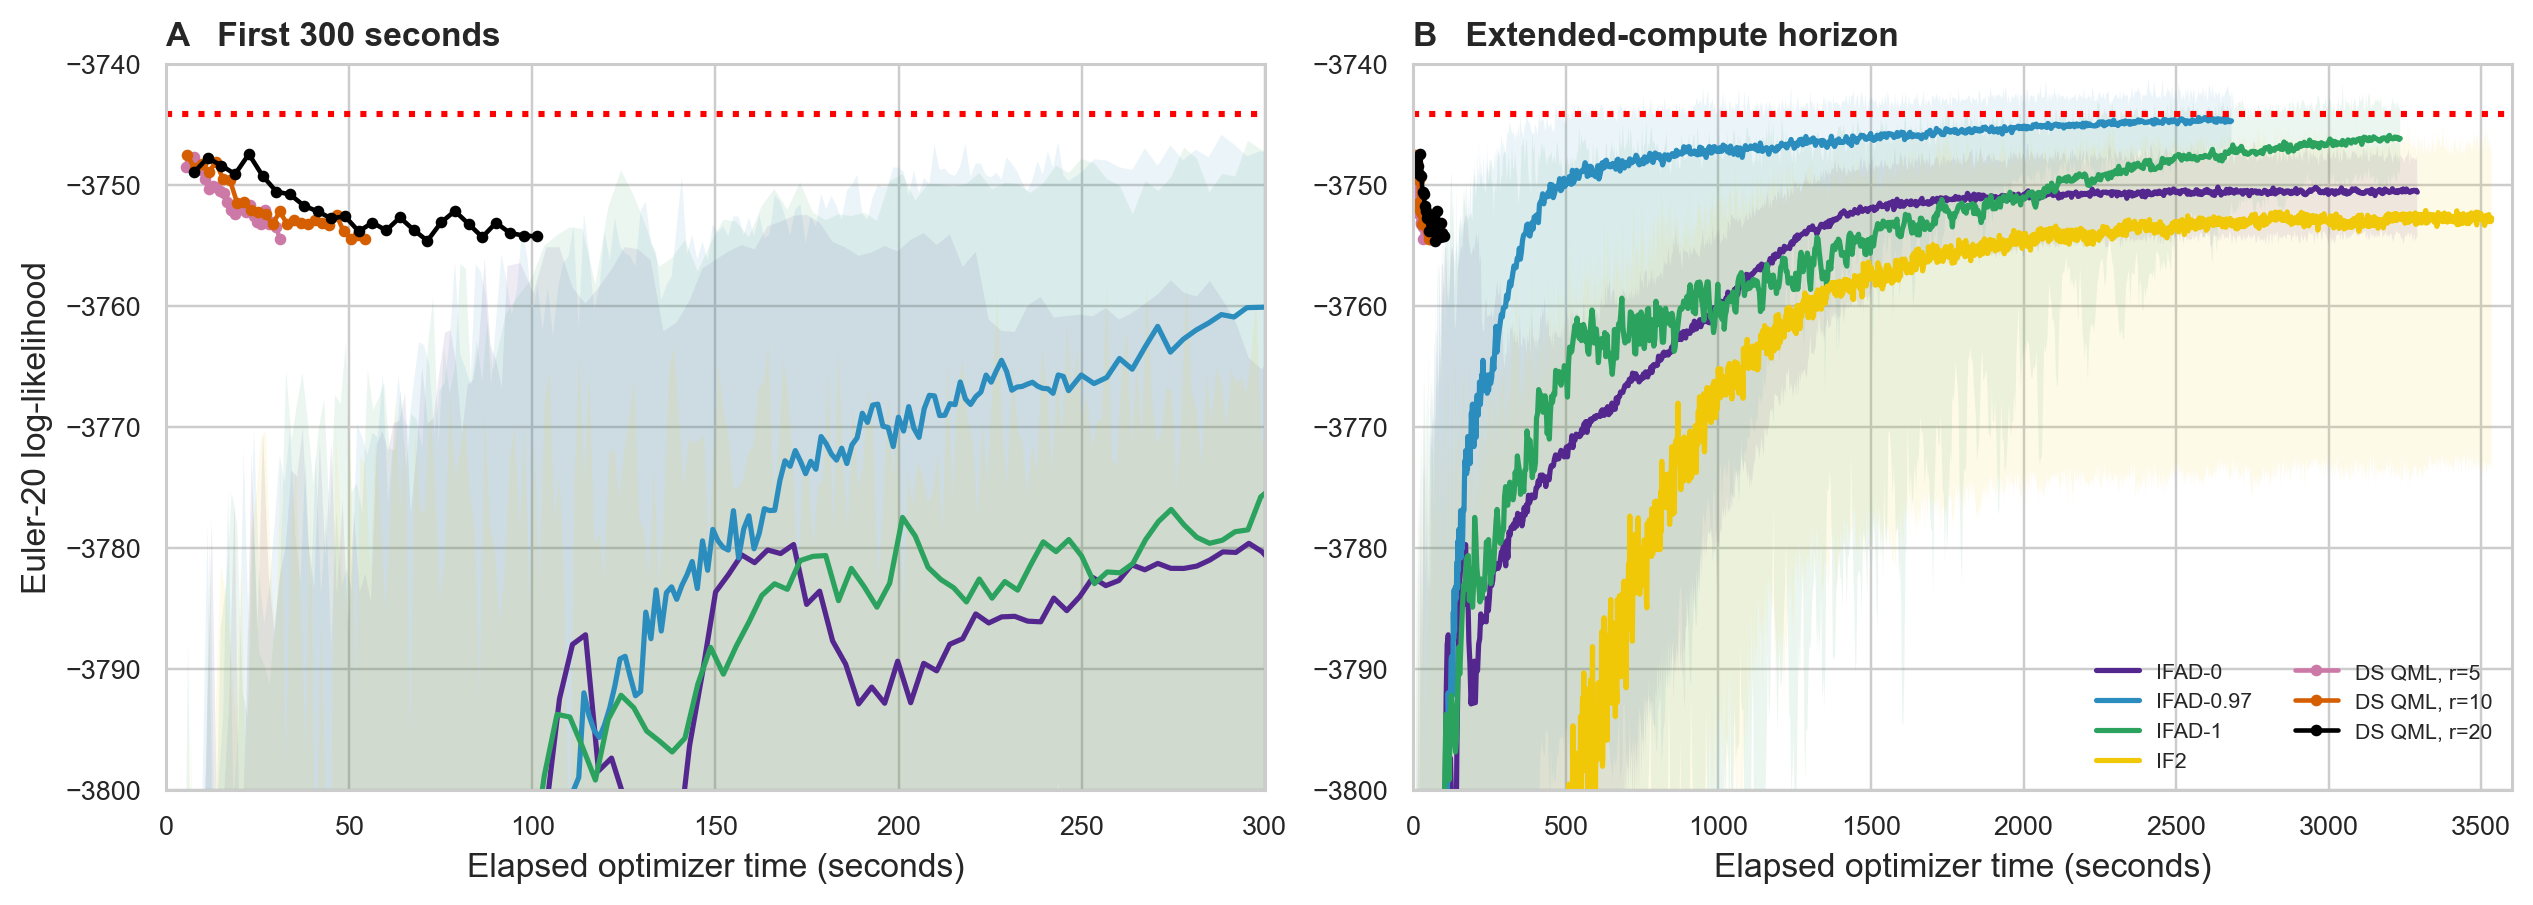
\includegraphics[width=\textwidth]{optimization_comparison.png}
\caption{Common-target optimization progress against elapsed time.  The four
DMOP curves reproduce the extended-compute manuscript traces (median with
10th-to-maximum envelope across 100 searches) using their unmonitored component
runtimes.  DS curves start at the favorable published point and show post-hoc
Euler-20 particle-filter evaluations at every optimizer iterate against the
measured DS optimizer time; monitoring time is excluded.  The DS Gaussian
criterion rises while the Euler-20 target generally falls.}
\label{fig:optimization}
\end{figure}

Across the monitored published-point paths, the Euler-20 likelihood changes by
$-5.98$, $-6.92$, and $-5.29$ log units for $r=5,10,20$, respectively, over
31, 54, and 101 seconds.  These changes show the surrogate-target mismatch
clearly, but their ordering is again nonmonotone and is not a test of
DS-SAEM genealogy degradation.

\begin{figure}[htbp]
\centering
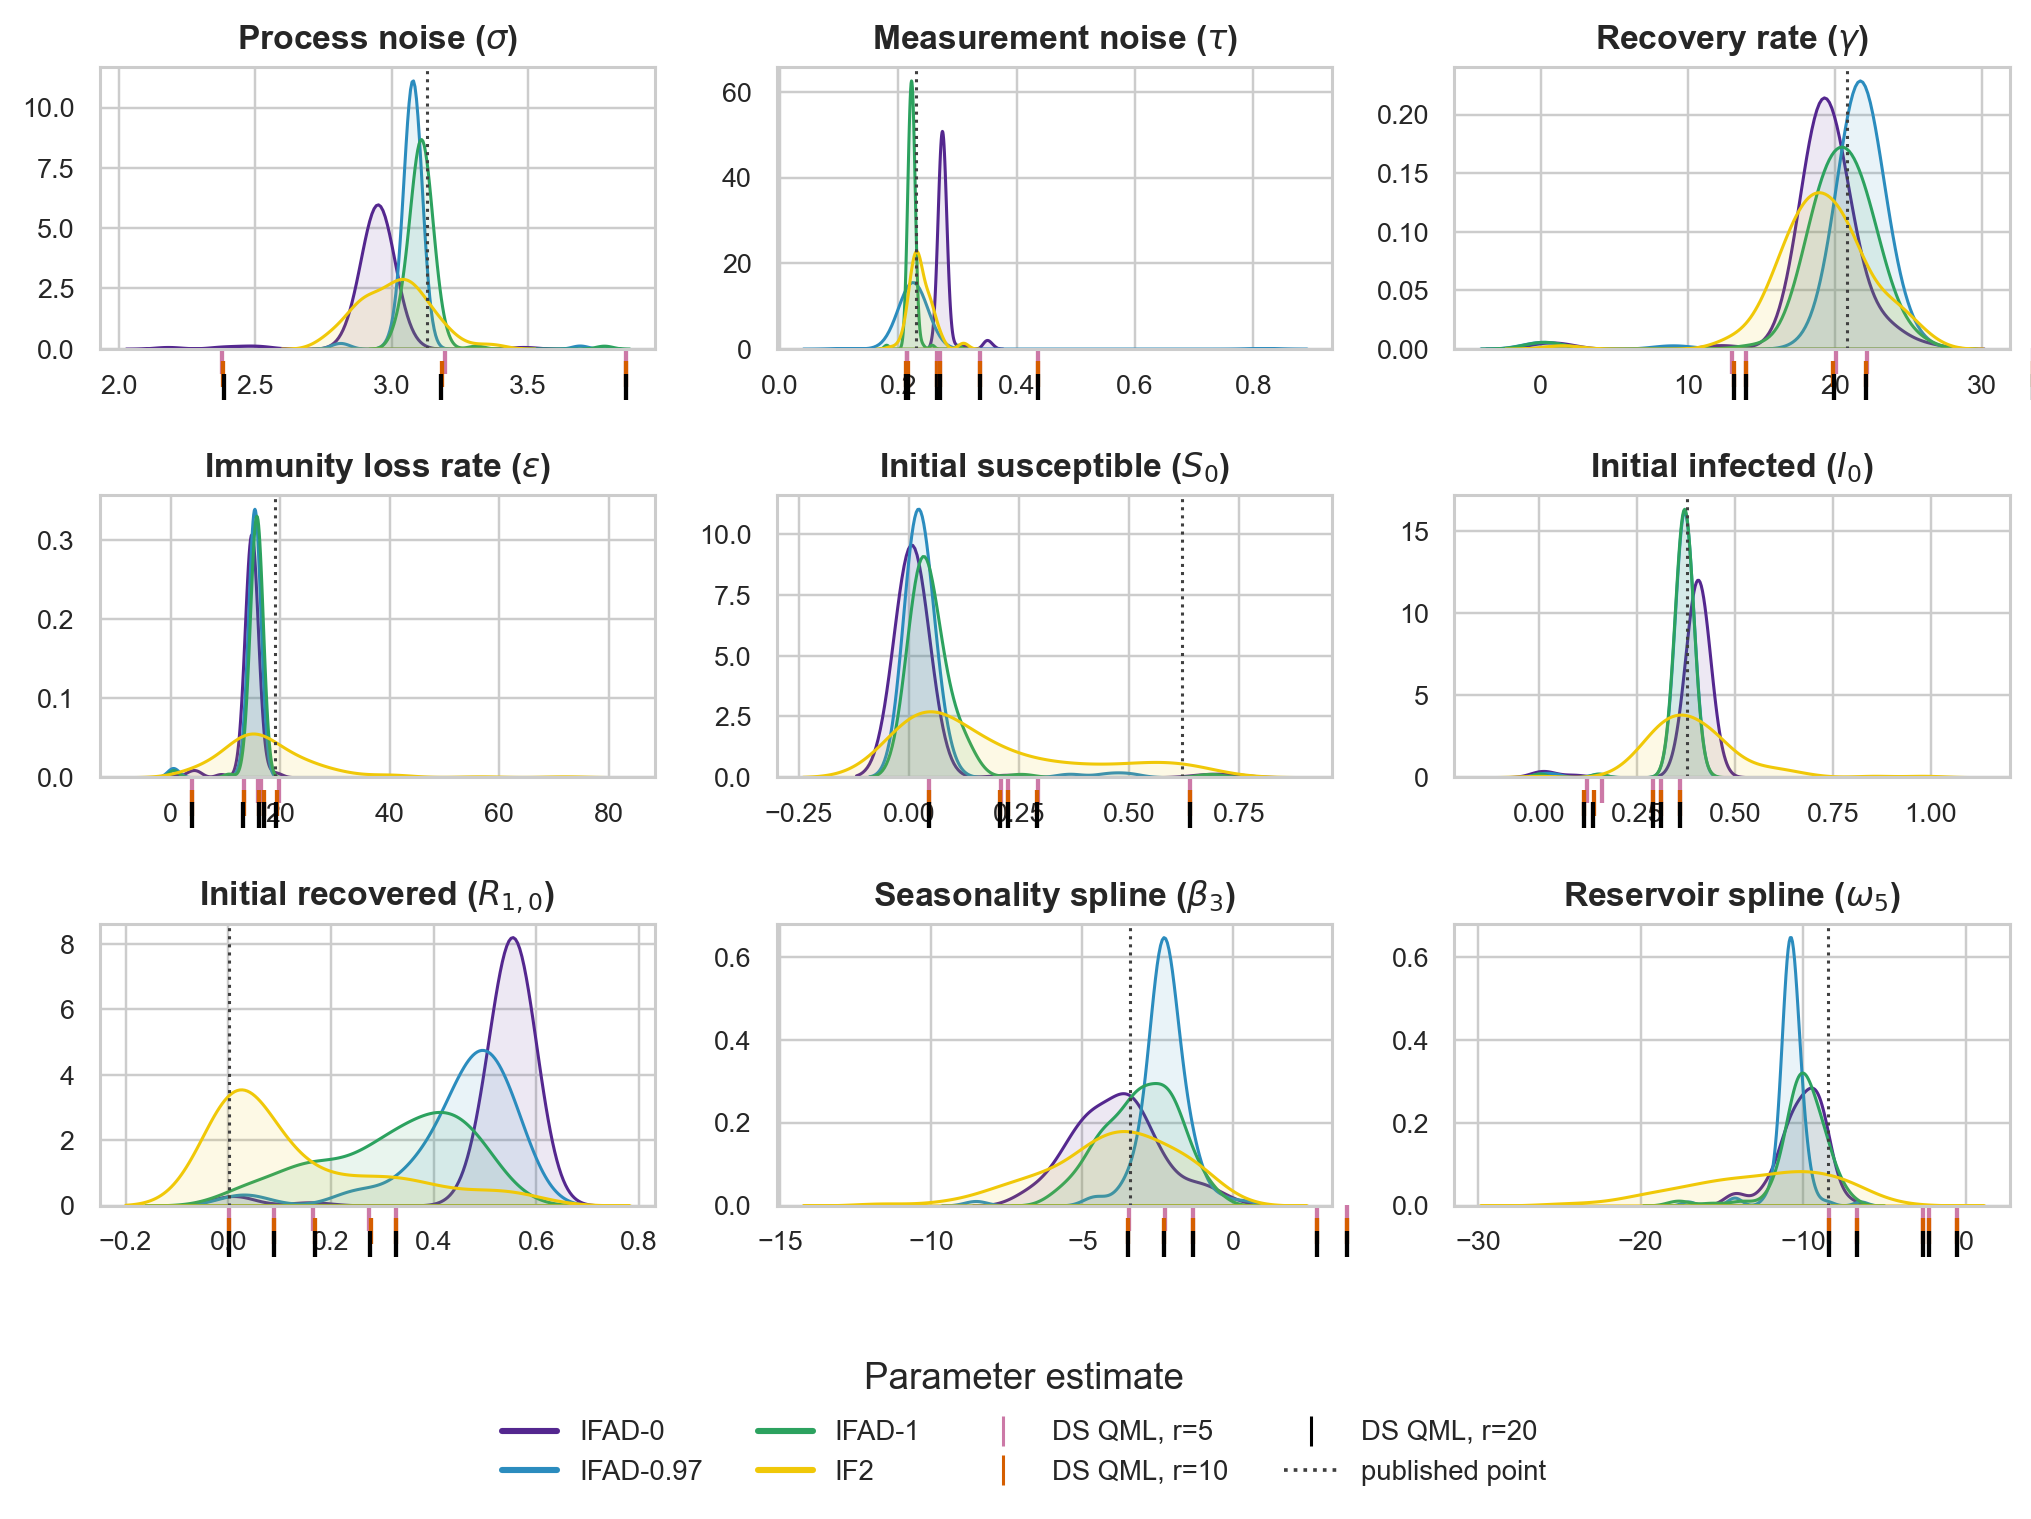
\includegraphics[width=\textwidth]{parameter_comparison.png}
\caption{Analogue of DMOP Figure~4 containing all four original extended-effort
methods and the DS-QML estimates.  Filled curves are the 100 manuscript
replicates per method.  Colored rug marks below each panel are the five DS
estimates for each inference grid; they are not turned into misleading density
estimates.  Dotted vertical lines mark the published starting point.}
\label{fig:parameters}
\end{figure}

\FloatBarrier

\section{Does Karppinen need to be combined with Ditlevsen?}

Not at the measurement scale for the reason proposed by the reviewer: when
$r=1$, there are no artificial within-month states for a bridge sampler to
repair.  KSV becomes relevant for $r>1$, where the ordinary backward kernel
concentrates as the local transition variance shrinks.  The stable block-
lookahead ESS shows that a KSV-style fixed-month block can address that
particular mixing mechanism.

It does not solve either remaining problem.  First, KSV cannot make a
first-bracket transition full-dimensional when the Dacca bracket chain is
longer.  Second, it cannot stabilize the coarse monthly DS Taylor mean.  A
coherent combined method needs a higher-bracket transition approximation, a
global time-varying linear-Gaussian auxiliary proposal, exact transition-density
correction potentials, and a numerical score or M-step.  The complete proposed
algorithm and correction formula are given in \texttt{../method.pdf}; the code
provides tested block-transition and Gaussian bridge-conditional routines.

\section{Conclusion and scope}

For this implementation, IFAD-$0.97$ outperforms every successful DS-local QML
fit by a practically large Euler-20 log-likelihood margin.  The best
25-iteration DS-local result is $-3753.86$, 9.69 log-likelihood units below the
paper's $-3744.17$; its best median over the tested grids is $-5913.45$, versus
$-3745.77$ for comparable-effort IFAD-$0.97$.  The five-start medians are a
scaled reliability check rather than a substitute for the paper's 100 runs,
but the failure of the wide-box starts to reach the high-likelihood region is
unambiguous.  More importantly,
the experiment identifies why the comparison is not simply ``DS at
$\Delta=1/20$ month'': coarse DS transitions are unstable, fine-grid ordinary
backward sampling degenerates, and Dacca requires more bracket levels than the
DS model class.

This is not a claim that every possible higher-order, bridge-blocked transition
density method must fail.  The full DS--Krylov--KSV stochastic-approximation
Fisher-score method specified in the companion note has not been run, so the
lookahead ESS is a
mechanism diagnostic rather than a parameter-estimation result for that full
algorithm.  The negative comparison applies to the implemented DS moment-QML
competitor, with all modifications and numerical regularization disclosed.

\end{document}
